\documentclass[a4paper,12pt,reqno,french]{article}

\usepackage{../utilities}

\newcounter{cptexo}
\newcommand{\exer}{\stepcounter{cptexo} {\LARGE Exercice \arabic{cptexo}} \vspace{1cm}}

\captionsetup[figure]{labelformat=empty}

\geometry{
	a4paper,
	total={170mm,257mm},
	left=20mm,
	right=20mm,
	top=20mm,
	bottom=20mm
}

\newcounter{cptquest}[cptexo]

\newtcolorbox{correc}{
		blanker,
		breakable,
		left=0mm,
		top=5mm,
		bottom=5mm,
		boxsep=0mm,
		borderline west={0.5mm}{-5mm}{teal8},
		enhanced, fonttitle=\bfseries,
		coltext=azure5,
		colback=white,
    detach title,
    overlay={
        \node[rotate=90, minimum width=1cm, anchor=south,yshift=0.75cm,blue3] at (frame.west) {\large Correction};
    }
}

\newtcolorbox{rqs}{
		blanker,
		breakable,
		left=0mm,
		top=5mm,
		bottom=5mm,
		boxsep=0mm,
		borderline west={0.5mm}{-5mm}{brown8},
		enhanced, fonttitle=\bfseries,
		coltext=brown6,
		colback=white,
    detach title,
    overlay={
        \node[rotate=90, minimum width=1cm, anchor=south,yshift=0.75cm,red2] at (frame.west) {\large Remarque(s)};
    }
}

\newtcolorbox{questionBox}[1]{
	blanker,
		breakable,
	left=6mm,
	top=1mm,
	bottom=1mm,
	enhanced,
	colback=white,
    overlay={
        \node[minimum width=1cm, xshift=-1cm,red5] at (frame.west) {\large \textbf{/ #1}};
    }
}

% envir super sensible à l'espacement de départ : coller le début de la question au début de l'env (sale certes, TODO à améliorer)
\newenvironment{question}[1]{
	\vspace{3mm}
	\begin{questionBox}{#1} \stepcounter{cptquest} \tikz[overlay]{
			\node at (-0.4,0.1) {\textbf{\arabic{cptquest})}};
		}}{
	\end{questionBox}
	\vspace{3mm}
}



\parindent=0mm

\begin{document}
	
	{
		
		\vspace*{7cm}
		{\fontsize{30}{40}\selectfont Correction DS}
		
		\vspace{5mm}
		{\fontsize{20}{30}\selectfont Limites et continuité de fonctions}
		
		\vspace{3cm}
		
		\Large
		Sujet qui commence par $f(x) = \frac{2x+3}{7-x}$
	}
	
	\newpage
	
	\exer
	
	Soit la fonction $f$ définie par l'expression $f(x) = \frac{2x+3}{7-x}$.
	
	\begin{question}{2}Calculer $\limite{x \to +\infty} f(x)$.
		
		Peut-on en déduire que la courbe représentative de $f$ admet une asymptote ?
		
		Si oui laquelle ?
	\end{question}
	
	\begin{correc}
		
		On factorise numérateur et dénominateur	dans l'expression de $f$ :
		
		\[
			f(x) = \frac{2x+3}{7-x} = \frac{x \cdot \left( 2+\frac{3}{x}\right)}{x \cdot \left(\frac{7}{x} - 1\right)} = \frac{2+\frac{3}{x}}{\frac{7}{x} - 1} \text{.}
		\]
		
		Comme $\limite{x \to +\infty} 2+\frac{3}{x} = 2$ et $\limite{x \to +\infty} \frac{7}{x} - 1 = -1$ alors par quotient de limites $\limite{x \to +\infty} f(x) = \frac{2}{-1} = -2$.
		
		On peut en déduire que la courbe représentative de $f$ admet une asymptote horizontale : la droite d'équation $y=-2$.
		
	\end{correc}
	
	\begin{rqs}
			
		\begin{itemize}
			
			\item Attention à bien regarder la limite en $+\infty$, il n'était dans cette question pas le moment de regarder « $x > 7$ donc $0 > 7-x$ etc ».
			
			\item Il s'agissait effectivement d'une forme indéterminée, il fallait donc lever l'indétermination en factorisant. \textbf{Remarque} : il est bien de faire remarquer la FI à l'écrit, mais pour ceux qui l'ont noté je pense que vous avez passé un certain temps à l'écrire, temps que vous n'avez pas pu investir dans les autres exercices.
			
			\item Attention aussi à ne pas avoir dans la parenthèse du dénominateur $1-\frac{7}{x}$ au lieu de $\frac{7}{x}-1$, ni $7-\frac{1}{x}$ ou $\frac{1}{x}-7$.
			
			\item Ça n'est pas $f$ qui admet une asymptote mais sa courbe représentative (notée $\mathscr C_f$ pour ceux qui ont la compréhensible atonie d'écrire toute l'expression).
			
			\item L'asymptote n'est pas « en $y=-2$ » ni « en $+\infty$ » (même si c'est l'idée) mais est une \underline{droite} d'équation $y=-2$.
			
		\end{itemize}
		
	\end{rqs}
	
	\begin{question}{2}Conjecturer si la courbe représentative de $f$ admet une asymptote \underline{verticale} (s'aider de la calculatrice).
		
		Si oui laquelle ?
		
	\end{question}
	
	
	\begin{correc}
		
		On peut conjecturer à l'aide de la calculatrice que la courbe représentative de $f$ admet la droite d'équation $x=7$ comme asymptote verticale.
		\vspace{-1cm}
		\begin{figure}[H]
		\end{figure}
		\begin{figure}[H]
			\centering
			\begin{minipage}{.5\textwidth}
				\centering
			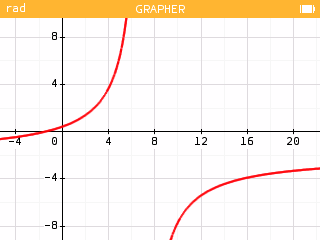
\includegraphics[width=0.9\textwidth]{scr1}
				\captionof{figure}{\centering La courbe semble monter autour d'une valeur proche de $8$.}
			\end{minipage}%
			\begin{minipage}{.5\textwidth}
				\centering
			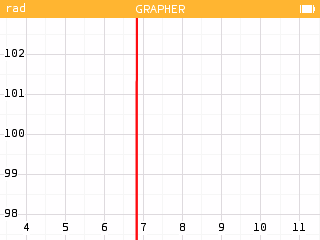
\includegraphics[width=0.9\textwidth]{scr2}
				\captionof{figure}{\centering Elle monte effectivement et plus précisément proche de $7$.}
			\end{minipage}
		\end{figure}
		
	\end{correc}
	
	\begin{rqs}
		
		\begin{itemize}
			
			\item Comme à la question précédente et à chaque fois que l'on parle d'asymptote : n'oublier ni \textbf{droite}, ni \textbf{verticale} (le cas échéant) ni son \textbf{équation}.
			
			\item L'expression de $f$ pouvait donner un indice : en regardant le dénominateur, c'est la valeur $x=7$ qui pose problème ; la fonction n'est pas définie en $7$ (elle y explose, c'est ce que l'on montre à la question précédente).
			
		\end{itemize}
		
	\end{rqs}
	
	\begin{question}{2}Confirmer la conjecture par un calcul de limite. \end{question}
	
	\begin{correc}
		
		On calcule $\limite{x \to 7^+} f(x)$.
		
		Lorsque $x>7$, $0>7-x$. Donc $\limite{x \to 7^+} 
		-x = 0^-$. De plus $\limite{x \to 7^+} 2x+3 = 17$.
		
		Ainsi par quotient de limites on a $\limite{x \to 7^+} f(x) = -\infty$.
		
		Ceci confirme la conjecture : $\mathscr C_f$ admet bien la droite d'équation $x=7$ comme asymptote verticale.
		
	\end{correc}
	
	\begin{rqs}
		
		\begin{itemize}
			
			\item On aurait pu calculer la limite en $7^-$, on aurait trouvé $+\infty$ mais ça n'aurait pas changé le résultat (on pouvait le faire en plus aussi, mais attention à la perte de temps par rapport à la longueur du sujet).
			
			\item Ne pas oublier de répondre à la question en concluant par une phrase. Un simple « Cela confirme la conjecture » suffisait.
			
		\end{itemize}
		
	\end{rqs}
	
	\exer
	
	Soit la fonction $h$ définie par l'expression $h(x)=e^x+2x+1$.
	
	\begin{question}{1}Déterminer la dérivée de $h$. \end{question}
	
	\begin{correc}
		
		La dérivée de $h$ est la fonction $h'$ définie par l'expression $h'(x)=e^x+2$.
		
	\end{correc}
	
	\begin{rqs}
		
		\begin{itemize}
			
			\item Attention à ne pas tomber dans le piège de confondre la dérivée de la fonction exponentielle avec celle de la fonction $x \mapsto x^n$. Cette erreur amenait à transformer $e^x$ en $xe^{x-1}$ en dérivant, erreur à ne plus reproduire !
			
			\item Autre petite erreur à ne plus commettre : dériver $2x$ en $x$ à la place de $2$.
			
		\end{itemize}
		
	\end{rqs}
	
	\begin{question}{1}Montrer que $h$ est strictement croissante. \end{question}
	
	\begin{correc}
		
		Comme $e^x > 0$ et $2>0$, on a $e^x+2 > 0$. Autrement dit $h'(x) > 0$, et donc (comme $h$ est continue) alors $h$ est strictement croissante.
		
	\end{correc}
	
	\begin{rqs}
		
		\begin{itemize}
			
			\item La remarque entre parenthèses « comme $h$ est continue » n'était pas nécessaire à citer pour obtenir tous les points. La précision est malgré cela importante car sans elle c'est faux de manière générale.
			
			\item La croissance au sens large (non stricte, avec un $\geq$), même si elle est vraie, ne permettait pas de conclure à la question suivante.
			
			\item Il est très bien de préciser que les opérations effectuées se déroulent sur $\R$. Il est tolérable de ne pas le préciser ici, c'est sous-entendu.
			
			\item Certains d'entres vous ont proposé une réponse argumentée. J'ai accordé une partie des points lorsque l'argumentation montrait un minimum de réflexion (donc à chaque fois il me semble).
			
			\item Ni $h$ ni sa dérivée ne sont des fonctions polynômes : ne pas partir dans un calcul de discriminant !
			
		\end{itemize}
		
	\end{rqs}
	
	\begin{question}{3,5}On admet que $h$ est continue sur $\R$.
	
	En déduire que l'équation $h(x)=8$ admet une \underline{unique} solution sur l'intervalle $[-10;10]$.
	
	\end{question}
	
	\begin{correc}
		
		On sait que :
		
		\textbullet \ $h$ est continue sur $\R$ donc sur $[-10;10]$ et strictement croissante.
		
		\textbullet \ $h(-10) \approx -19$ et $h(10) \approx 22047$, donc $h(-10) \leq 8 \leq h(10)$.
		
		Donc d'après le théorème des valeurs intermédiaires (TVI) monotone l'équation $h(x)=8$ admet une unique solution sur $[-10;10]$.
		
	\end{correc}
	
	\begin{rqs}
		
		\begin{itemize}
			
			\item Ne pas oublier la \textbf{stricte} croissance en hypothèse : c'est elle qui garantit l'unicité de la solution.
			
			\item Ne pas non plus oublier que c'est du TVI monotone dont il s'agit et non du simple TVI.
			
			\item Il faut me montrer que vous avez bien calculé $h(-10)$ et $h(10)$, que vous ne vous contentez pas simplement de l'écrire sans le vérifier.
			
			\item Ne pas écrire $h(-10) \leq h(x)=8 \leq h(10)$ mais plutôt $h(-10) \leq 8 \leq h(10)$. $h(x)=8$ est une équation, cela n'a pas \textit{officiellement} de sens de la mettre dans une inéquation.
			
		\end{itemize}
		
	\end{rqs}
	
	\exer
	
	On considère la fonction $g$ définie par l'expression $g(x)=x^3-x^2-x+1$.
	
	\begin{question}{2}Calculer les limites en $+\infty$ et en $-\infty$ de $g$. \end{question}
	
	\begin{correc}
		
		On commence par factoriser l'expression de $g$ :
		
		\[
			g(x) = x^3-x^2-x+1 = x^3 \cdot \left( 1 - \frac{1}{x} - \frac{1}{x^2} + \frac{1}{x^3} \right) \text{.}
		\]
		
		\underline{En $+\infty$}
		
		D'une part $\limite{x \to +\infty} x^3 = +\infty$.
		
		D'autre part, $\limite{x \to +\infty} \left( 1 - \frac{1}{x} - \frac{1}{x^2} + \frac{1}{x^3} \right) = 1$ (par somme de limites).
		
		Donc par produit de limites $\limite{x \to +\infty} g(x) = +\infty$.
		
		\underline{En $-\infty$}
		
		D'une part $\limite{x \to -\infty} x^3 = -\infty$.
		
		D'autre part, $\limite{x \to +\infty} \left( 1 - \frac{1}{x} - \frac{1}{x^2} + \frac{1}{x^3} \right) = 1$ (par somme de limites).
		
		Donc par produit de limites $\limite{x \to -\infty} g(x) = -\infty$.
		
	\end{correc}
	
	\begin{rqs}
		
		\begin{itemize}
				
			\item Le « par somme de limites » entre parenthèses n'était pas essentiel : c'est le « par produit de limites » que l'on applique en dernier et donc surtout lui que j'attendais (mais mettre la justification pour la somme était très bien).
			
			\item Ne pas oublier le signe $-$ qui se balade pour la limite finale en $-\infty$.
			
		\end{itemize}
		
	\end{rqs}
	
	\begin{question}{3}Étudier les variations de la fonction $g$ puis dresser son tableau de variations. \end{question}
	
	\begin{correc}
		
		On dérive d'abord $g$ : $g'(x) = 3x^2-2x-1$.
		
		On détermine le signe de $g'$ en déterminant les racines de cette fonction polynôme.
		
		$\Delta = (-2)^2-4 \times 3 \times (-1) = 4+12 = 16$. La fonction $g'$ possède deux racines :
		
		$\frac{-(-2)-\sqrt{\Delta}}{2 \times 3} = \frac{-2}{6} = -\frac{1}{3}$ et $\frac{-(-2)+\sqrt{\Delta}}{2 \times 3} = \cdots = 1$.
		
		On en déduit le tableau de signe / variations suivant :
		
		% TODO Même rq qu'à chaque fois : paquet tds et tdv à construire
		\begin{figure}[H]
			\centering
			\begin{tikzpicture}
				
				\draw[azure5] (0,0) rectangle (8,5);
				
				\draw[azure5] (0,2) -- (8,2);
				\draw[azure5] (0,4) -- (8,4);
				\draw[azure5] (2,0) -- (2,5);
				
				\node[azure5] at (1,4.5) {$x$};
				\node[align=center,azure5] at (1,3) {Signe \\ de $g'$};
				\node[align=center,azure5] at (1,1) {Variations \\ de $g$};
				
				
				\draw[azure5] (4,2) -- (4,4);
				\draw[azure5] (6,2) -- (6,4);
				
				\node[azure5] at (4,4.5) {$-1/3$};
				\node[azure5] at (6,4.5) {$1$};
				
				\node[azure5,anchor=west] at (2,4.5) {$-\infty$};
				\node[azure5,anchor=east] at (8,4.5) {$+\infty$};
				
				\node[azure5] at (3,3) {\Large $+$};
				\node[azure5] at (5,3) {\Large $-$};
				\node[azure5] at (7,3) {\Large $+$};
				
				\draw[azure5,->] (2.75,0.75) -- (3.25,1.25);
				\draw[azure5,->] (4.75,1.25) -- (5.25,0.75);
				\draw[azure5,->] (6.75,0.75) -- (7.25,1.25);
				
				\node[azure5,anchor=south west] at (2,0) {$-\infty$};
				\node[azure5,anchor=north east] at (8,2) {$+\infty$};
				
				\node[azure5] at (4,1.5) {$\approx 1,19$};
				\node[azure5] at (6,0.5) {$0$};
				
			\end{tikzpicture}
		\end{figure}
		
	\end{correc}
	
	\begin{rqs}
		
		\begin{itemize}
			
			\item Ne pas oublier de rajouter les limites en $+\infty$ en $-\infty$ dans le tableau (calculées dans la première question).
			
			\item Source d'erreurs : la calcul du discriminant et des racines. Cela demandait certains calculs qui pouvaient amener certaines erreurs.
			
			\item Signe du coefficient devant $x^2$ à l'exterieur des racines : $3$ est positif donc $+$ en dehors de $[-1/3;1]$ et $-$ à l'interieur.
			
			\item Il n'était pas nécessaire de calculer $g(-1/3)$ et $g(1)$ à cette question et les mettre dans le tableau mais ces valeurs étaient presque nécessaires pour répondre à la question qui suit.
			
			\item Si à la première question vous trouviez par exemple $\limite{x \to +\infty} g(x) = -\infty$ le tableau vous indiquait votre mauvaise réponse : la fonction ne peut pas croître et tendre vers $-\infty$ !
			
			\item Certains n'ont pas correctement calculé $g(-1/3)$ à la calculatrice : attention aux parenthèses et au signe (surtout pour le $-\left( - \frac{1}{3}\right)^2$.
			
		\end{itemize}
		
	\end{rqs}
	
	\begin{question}{3,5}Montrer que l'équation $g(x)=1$ admet \underline{au moins} trois solutions sur $\R$. \end{question}
	
	\begin{correc}
		
		On applique le théorème des valeurs intermédiaires sur l'intervalle $[-10;-1/3]$.
		
		On sait que :
		
		\textbullet \ $g$ est continue sur $[-10;-1/3]$ car est une fonction polynôme.
		
		\textbullet \ $g(-10) = -1089$ et $g(-1/3) \approx 1,19$, donc $g(-10) \leq 1 \leq g(-1/3)$.
		
		Donc d'après le TVI, l'équation $g(x)=1$ admet au moins une solution sur l'intervalle $[-10;-1/3]$.
		
		On applique à nouveau le TVI sur les intervalles $[-1/3;1]$ et $[1;10]$ ($1,19 \geq 1 \geq 0$ et $0 \leq 1 \leq g(10)$ où $g(10) = 891$).
		
		Ainsi l'équation $g(x)=1$ admet au moins trois solutions sur $\R$.
		
	\end{correc}
	
	\begin{rqs}
		
		\begin{itemize}
			
			\item Si vous aviez le temps c'est bien d'avoir rédigé trois fois en entier l'application du TVI, cependant ce que j'ai écrit en correction suffisait. Montrez une fois que vous savez très bien le rédiger et pas besoin de ré-écrire presque la même chose deux nouvelles fois.
			
			\item Les $-10$ et $10$ ont été choisis car ils permettaient d'appliquer le TVI. $-100$ et $100$ fonctionnaient aussi, ou encore $-1000$ et $1000$ etc.
			
		\end{itemize}
		
	\end{rqs}
	
	
	
	
	
	
	
	
	
	
	
	
	
	
	
	
	
	
	% Sujet 2
	
	
	
	
	
	
	
	
	
	
	
	
	
	
	
	
	
	
	\newpage
	{
		
		\vspace*{7cm}
		{\fontsize{30}{40}\selectfont Correction DS}
		
		\vspace{5mm}
		{\fontsize{20}{30}\selectfont Limites et continuité de fonctions}
		
		\vspace{3cm}
		
		\Large
		Sujet qui commence par $f(x) = \frac{3x+2}{4-x}$
	}
	
	\newpage
	
	\exer
	
	Soit la fonction $f$ définie par l'expression $f(x) = \frac{3x+2}{4-x}$.
	
	\begin{question}{2}Calculer $\limite{x \to +\infty} f(x)$.
		
		Peut-on en déduire que la courbe représentative de $f$ admet une asymptote ?
		
		Si oui laquelle ?
	\end{question}
	
	\begin{correc}
		
		On factorise numérateur et dénominateur	dans l'expression de $f$ :
		
		\[
			f(x) = \frac{3x+2}{4-x} = \frac{x \cdot \left( 3+\frac{2}{x}\right)}{x \cdot \left(\frac{4}{x} - 1\right)} = \frac{3+\frac{2}{x}}{\frac{4}{x} - 1} \text{.}
		\]
		
		Comme $\limite{x \to +\infty} 3+\frac{2}{x} = 3$ et $\limite{x \to +\infty} \frac{4}{x} - 1 = -1$ alors par quotient de limites $\limite{x \to +\infty} f(x) = \frac{3}{-1} = -3$.
		
		On peut en déduire que la courbe représentative de $f$ admet une asymptote horizontale : la droite d'équation $y=-3$.
		
	\end{correc}
	
	\begin{rqs}
			
		\begin{itemize}
			
			\item Attention à bien regarder la limite en $+\infty$, il n'était dans cette question pas le moment de regarder « $x > 4$ donc $0 > 4-x$ etc ».
			
			\item Il s'agissait effectivement d'une forme indéterminée, il fallait donc lever l'indétermination en factorisant. \textbf{Remarque} : il est bien de faire remarquer la FI à l'écrit, mais pour ceux qui l'ont noté je pense que vous avez passé un certain temps à l'écrire, temps que vous n'avez pas pu investir dans les autres exercices.
			
			\item Attention aussi à ne pas avoir dans la parenthèse du dénominateur $1-\frac{4}{x}$ au lieu de $\frac{4}{x}-1$, ni $4-\frac{1}{x}$ ou $\frac{1}{x}-4$.
			
			\item Ça n'est pas $f$ qui admet une asymptote mais sa courbe représentative (notée $\mathscr C_f$ pour ceux qui ont la compréhensible atonie d'écrire toute l'expression).
			
			\item L'asymptote n'est pas « en $y=-3$ » ni « en $+\infty$ » (même si c'est l'idée) mais est une \underline{droite} d'équation $y=-3$.
			
		\end{itemize}
		
	\end{rqs}
	
	\begin{question}{2}Conjecturer si la courbe représentative de $f$ admet une asymptote \underline{verticale} (s'aider de la calculatrice).
		
		Si oui laquelle ?
		
	\end{question}
	
	
	\begin{correc}
		
		On peut conjecturer à l'aide de la calculatrice que la courbe représentative de $f$ admet la droite d'équation $x=4$ comme asymptote verticale.
		\vspace{-1cm}
		\begin{figure}[H]
		\end{figure}
		\begin{figure}[H]
			\centering
			\begin{minipage}{.5\textwidth}
				\centering
			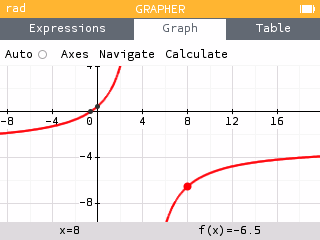
\includegraphics[width=0.9\textwidth]{scr1bis}
				\captionof{figure}{\centering La courbe semble monter autour d'une valeur proche de $4$.}
			\end{minipage}%
			\begin{minipage}{.5\textwidth}
				\centering
			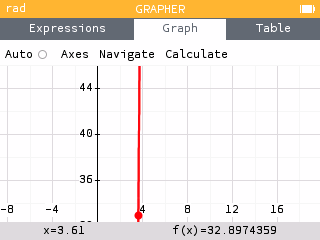
\includegraphics[width=0.9\textwidth]{scr2bis}
				\captionof{figure}{\centering Elle monte effectivement et précisément proche de $4$.}
			\end{minipage}
		\end{figure}
		
	\end{correc}
	
	\begin{rqs}
		
		\begin{itemize}
			
			\item Comme à la question précédente et à chaque fois que l'on parle d'asymptote : n'oublier ni \textbf{droite}, ni \textbf{verticale} (le cas échéant) ni son \textbf{équation}.
			
			\item L'expression de $f$ pouvait donner un indice : en regardant le dénominateur, c'est la valeur $x=4$ qui pose problème ; la fonction n'est pas définie en $4$ (elle y explose, c'est ce que l'on montre à la question précédente).
			
		\end{itemize}
		
	\end{rqs}
	
	\begin{question}{2}Confirmer la conjecture par un calcul de limite. \end{question}
	
	\begin{correc}
		
		On calcule $\limite{x \to 4^+} f(x)$.
		
		Lorsque $x>4$, $0>4-x$. Donc $\limite{x \to 4^+} 
		-x = 0^-$. De plus $\limite{x \to 4^+} 3x+2 = 14$.
		
		Ainsi par quotient de limites on a $\limite{x \to 4^+} f(x) = -\infty$.
		
		Ceci confirme la conjecture : $\mathscr C_f$ admet bien la droite d'équation $x=4$ comme asymptote verticale.
		
	\end{correc}
	
	\begin{rqs}
		
		\begin{itemize}
			
			\item On aurait pu calculer la limite en $4^-$, on aurait trouvé $+\infty$ mais ça n'aurait pas changé le résultat (on pouvait le faire en plus aussi, mais attention à la perte de temps par rapport à la longueur du sujet).
			
			\item Ne pas oublier de répondre à la question en concluant par une phrase. Un simple « Cela confirme la conjecture » suffisait.
			
		\end{itemize}
		
	\end{rqs}
	
	\exer
	
	Soit la fonction $h$ définie par l'expression $h(x)=e^x+x+12$.
	
	\begin{question}{1}Déterminer la dérivée de $h$. \end{question}
	
	\begin{correc}
		
		La dérivée de $h$ est la fonction $h'$ définie par l'expression $h'(x)=e^x+1$.
		
	\end{correc}
	
	\begin{rqs}
		
		Attention à ne pas tomber dans le piège de confondre la dérivée de la fonction exponentielle avec celle de la fonction $x \mapsto x^n$. Cette erreur amenait à transformer $e^x$ en $xe^{x-1}$ en dérivant, erreur à ne plus reproduire !
		
	\end{rqs}
	
	\begin{question}{1}Montrer que $h$ est strictement croissante. \end{question}
	
	\begin{correc}
		
		Comme $e^x > 0$ et $1>0$, on a $e^x+1 > 0$. Autrement dit $h'(x) > 0$, et donc (comme $h$ est continue) alors $h$ est strictement croissante.
		
	\end{correc}
	
	\begin{rqs}
		
		\begin{itemize}
			
			\item La remarque entre parenthèses « comme $h$ est continue » n'était pas nécessaire à citer pour obtenir tous les points. La précision est malgré cela importante car sans elle c'est faux de manière générale.
			
			\item La croissance au sens large (non stricte, avec un $\geq$), même si elle est vraie, ne permettait pas de conclure à la question suivante.
			
			\item Il est très bien de préciser que les opérations effectuées se déroulent sur $\R$. Il est tolérable de ne pas le préciser ici, c'est sous-entendu.
			
			\item Certains d'entres vous ont proposé une réponse argumentée. J'ai accordé une partie des points lorsque l'argumentation montrait un minimum de réflexion (donc à chaque fois il me semble).
			
			\item Ni $h$ ni sa dérivée ne sont des fonctions polynômes : ne pas partir dans un calcul de discriminant !
			
		\end{itemize}
		
	\end{rqs}
	
	\begin{question}{3,5}On admet que $h$ est continue sur $\R$.
	
	En déduire que l'équation $h(x)=20$ admet une \underline{unique} solution sur l'intervalle $[0;10]$.
	
	\end{question}
	
	\begin{correc}
		
		On sait que :
		
		\textbullet \ $h$ est continue sur $\R$ donc sur $[0;10]$ et strictement croissante.
		
		\textbullet \ $h(0) =-12 $ et $h(10) \approx 22048$, donc $h(0) \leq 20 \leq h(10)$.
		
		Donc d'après le théorème des valeurs intermédiaires (TVI) monotone l'équation $h(x)=20$ admet une unique solution sur $[0;10]$.
		
	\end{correc}
	
	\begin{rqs}
		
		\begin{itemize}
			
			\item Ne pas oublier la \textbf{stricte} croissance en hypothèse : c'est elle qui garantit l'unicité de la solution.
			
			\item Ne pas non plus oublier que c'est du TVI monotone dont il s'agit et non du simple TVI.
			
			\item Il faut me montrer que vous avez bien calculé $h(0)$ et $h(10)$, que vous ne vous contentez pas simplement de l'écrire sans le vérifier.
			
			\item Ne pas écrire $h(0) \leq h(x)=20 \leq h(10)$ mais plutôt $h(0) \leq 20 \leq h(10)$. $h(x)=20$ est une équation, cela n'a pas \textit{officiellement} de sens de la mettre dans une inéquation.
			
		\end{itemize}
		
	\end{rqs}
	
	\exer
	
	On considère la fonction $g$ définie par l'expression $g(x)=-x^3+x^2+x-1$.
	
	\begin{question}{2}Calculer les limites en $+\infty$ et en $-\infty$ de $g$. \end{question}
	
	\begin{correc}
		
		On commence par factoriser l'expression de $g$ :
		
		\[
			g(x) = -x^3+x^2+x-1 = x^3 \cdot \left( -1 + \frac{1}{x} + \frac{1}{x^2} - \frac{1}{x^3} \right) \text{.}
		\]
		
		\underline{En $+\infty$}
		
		D'une part $\limite{x \to +\infty} x^3 = +\infty$.
		
		D'autre part, $\limite{x \to +\infty} \left( -1 + \frac{1}{x} + \frac{1}{x^2} - \frac{1}{x^3} \right) = -1$ (par somme de limites).
		
		Donc par produit de limites $\limite{x \to +\infty} g(x) = -\infty$.
		
		\underline{En $-\infty$}
		
		D'une part $\limite{x \to -\infty} x^3 = -\infty$.
		
		D'autre part, $\limite{x \to +\infty} \left( -1 + \frac{1}{x} + \frac{1}{x^2} - \frac{1}{x^3} \right) = -$ (par somme de limites).
		
		Donc par produit de limites $\limite{x \to -\infty} g(x) = +\infty$.
		
	\end{correc}
	
	\begin{rqs}
		
		\begin{itemize}
				
			\item Le « par somme de limites » entre parenthèses n'était pas essentiel : c'est le « par produit de limites » que l'on applique en dernier et donc surtout lui que j'attendais (mais mettre la justification pour la somme était très bien).
			
			\item Ne pas oublier le signe $-$ qui se balade pour la limite finale en $-\infty$ ($-$ par $-$ font $+$ pour la règle des signes).
			
		\end{itemize}
		
	\end{rqs}
	
	\begin{question}{3}Étudier les variations de la fonction $g$ puis dresser son tableau de variations. \end{question}
	
	\begin{correc}
		
		On dérive d'abord $g$ : $g'(x) = -3x^2+2x+1$.
		
		On détermine le signe de $g'$ en déterminant les racines de cette fonction polynôme.
		
		$\Delta = 2^2-4 \times (-3) \times 1 = 4+12 = 16$. La fonction $g'$ possède deux racines :
		
		$\frac{-2-\sqrt{\Delta}}{2 \times (-3)} = \frac{-6}{-6} = 1$ et $\frac{-2+\sqrt{\Delta}}{2 \times (-3)} = \cdots = -\frac{1}{3}$.
		
		On en déduit le tableau de signe / variations suivant :
		
		% TODO Même rq qu'à chaque fois : paquet tds et tdv à construire
		\begin{figure}[H]
			\centering
			\begin{tikzpicture}
				
				\draw[azure5] (0,0) rectangle (8,5);
				
				\draw[azure5] (0,2) -- (8,2);
				\draw[azure5] (0,4) -- (8,4);
				\draw[azure5] (2,0) -- (2,5);
				
				\node[azure5] at (1,4.5) {$x$};
				\node[align=center,azure5] at (1,3) {Signe \\ de $g'$};
				\node[align=center,azure5] at (1,1) {Variations \\ de $g$};
				
				
				\draw[azure5] (4,2) -- (4,4);
				\draw[azure5] (6,2) -- (6,4);
				
				\node[azure5] at (4,4.5) {$-1/3$};
				\node[azure5] at (6,4.5) {$1$};
				
				\node[azure5,anchor=west] at (2,4.5) {$-\infty$};
				\node[azure5,anchor=east] at (8,4.5) {$+\infty$};
				
				\node[azure5] at (3,3) {\Large $-$};
				\node[azure5] at (5,3) {\Large $+$};
				\node[azure5] at (7,3) {\Large $-$};
				
				\draw[azure5,->] (2.75,1.25) -- (3.25,0.75);
				\draw[azure5,->] (4.75,0.75) -- (5.25,1.25);
				\draw[azure5,->] (6.75,1.25) -- (7.25,0.75);
				
				\node[azure5,anchor=north west] at (2,2) {$+\infty$};
				\node[azure5,anchor=south east] at (8,0) {$-\infty$};
				
				\node[azure5] at (4,0.5) {$\approx -1,19$};
				\node[azure5] at (6,1.5) {$0$};
				
			\end{tikzpicture}
		\end{figure}
		
	\end{correc}
	
	\begin{rqs}
		
		\begin{itemize}
			
			\item Ne pas oublier de rajouter les limites en $+\infty$ en $-\infty$ dans le tableau (calculées dans la première question).
			
			\item Source d'erreurs : la calcul du discriminant et des racines. Cela demandait certains calculs qui pouvaient amener certaines erreurs.
			
			\item Signe du coefficient devant $x^2$ à l'exterieur des racines : $-3$ est positif donc $-$ en dehors de $[-1/3;1]$ et $+$ à l'interieur.
			
			\item Il n'était pas nécessaire de calculer $g(-1/3)$ et $g(1)$ à cette question et les mettre dans le tableau mais ces valeurs étaient presque nécessaires pour répondre à la question qui suit.
			
			\item Si à la première question vous trouviez par exemple $\limite{x \to +\infty} g(x) = +\infty$ le tableau vous indiquait votre mauvaise réponse : la fonction ne peut pas décroître et tendre vers $+\infty$ !
			
			\item Certains n'ont pas correctement calculé $g(-1/3)$ à la calculatrice : attention aux parenthèses et au signe (surtout pour le $+\left( - \frac{1}{3}\right)^2$).
			
		\end{itemize}
		
	\end{rqs}
	
	\begin{question}{3,5}Montrer que l'équation $g(x)=-1$ admet \underline{au moins} trois solutions sur $\R$. \end{question}
	
	\begin{correc}
		
		On applique le théorème des valeurs intermédiaires sur l'intervalle $[-10;-1/3]$.
		
		On sait que :
		
		\textbullet \ $g$ est continue sur $[-10;-1/3]$ car est une fonction polynôme.
		
		\textbullet \ $g(-10) = 1089$ et $g(-1/3) \approx -1,19$, donc $g(-10) \geq -1 \leq g(-1/3)$.
		
		Donc d'après le TVI, l'équation $g(x)=-1$ admet au moins une solution sur l'intervalle $[-10;-1/3]$.
		
		On applique à nouveau le TVI sur les intervalles $[-1/3;1]$ et $[1;10]$ ($-1,19 \leq -1 \leq 0$ et $0 \geq -1 \geq g(10)$ où $g(10) = -891$).
		
		Ainsi l'équation $g(x)=-1$ admet au moins trois solutions sur $\R$.
		
	\end{correc}
	
	\begin{rqs}
		
		\begin{itemize}
			
			\item Si vous aviez le temps c'est bien d'avoir rédigé trois fois en entier l'application du TVI, cependant ce que j'ai écrit en correction suffisait. Montrez une fois que vous savez très bien le rédiger et pas besoin de ré-écrire presque la même chose deux nouvelles fois.
			
			\item Les $-10$ et $10$ ont été choisis car ils permettaient d'appliquer le TVI. $-100$ et $100$ fonctionnaient aussi, ou encore $-1000$ et $1000$ etc.
			
		\end{itemize}
		
	\end{rqs}
	
	
	
	
	
	
	
\end{document}